\section{Description}\label{description}
\subsection{General Design}\label{general-design}

To address software design issues of existing and concurrent code bases,
such as DomainBed~\cite{domainbed2022github, gulrajani2020search} and Dassl~\cite{dassl2022github, zhou2021domain},
and to maximally decouple factors that might affect the performance of
domain generalization algorithms, we designed DomainLab with the
following features.

The package is closed to modification and open to extension.

The package offers the user a standalone application to specify the data
with data split protocol and preprocessing. To test an algorithm's
performance on a user's custom data, there is no need to change any code
across different files of the codebase anymore. The user only needs to
specify custom Python configuration file to incorporate their data.

Domain generalization algorithms were implemented with a transparent
underlying neural network architecture. The concrete neural network
architecture can thus be replaced by plugging in an architecture
implemented in a Python file or by specifying some of the already
implemented architectures, such as AlexNet~\cite{krizhevskyImageNetClassificationDeep2012}, via command line
arguments.

Selection of algorithms and neural network components are done via the
chain-of-responsibility method~\cite{gamma1995design}. Other design
patterns, including the observer pattern, visitor pattern, etc., are
also used to improve the decoupling of different factors contributing to
the performance of an algorithm (see also Section ``Components'' below).

With the above design, DomainLab offers users the flexibility to
construct custom tasks with their data, write custom neural network
architectures for use with the already implemented domain generalization
algorithms, and construct their domain generalization algorithms on top
of the existing components by specifying a Python file with custom
models and loss functions.

\subsection{Components}\label{components}

We used the following components to achieve the above design goals of
decoupling as depicted in \autoref{fig:cdiagram}.

\emph{Models} refer to a PyTorch module with a specified loss function
containing regularization effects of several domains and task-specific
losses (e.g., cross-entropy loss for classification tasks). The user can
configure the exact neural network architecture via command line
arguments. To extend DomainLab with new models, the user only needs to
specify a Python file defining the custom loss function while remaining
flexible with respect to the exact neural network used for each
submodule. The common classification loss calculation is done via a
parent model class. Thus, the individual models (e.g., representing
different domain regularization) can be reused for other tasks (e.g.,
segmentation) by simply inheriting another task loss.

\emph{Tasks} refer to a component where the user specifies different
datasets from different domains and preprocessing steps. There are
several types of tasks in DomainLab: (1) Built-in tasks, e.g.,
Color-Mnist, subsampled version of PACS, VLCS, etc., to provide a test
utility for algorithms. (2) ``TaskFolder,'' which can be used if the
data is already organized in a root folder with different subfolders
containing data from different domains and a further level of
sub-subfolders containing data from different classes. (3)
``TaskPathFile,'' which allows the user to specify each domain in a text
file indicating the path and label for each observation so that the user
can choose which portion of the sample to use for training, validation,
and testing.

\emph{Trainer} is the component that directs data flow to the model to
calculate the losses and update the model parameters. Several models can
share a common trainer. A specific trainer can also be a \emph{Visitor}
to models to update models' hyper-parameters like the weight to
regularization loss during training and implement techniques such as
warm-up, which follows the visitor design pattern from software
engineering.

Following the \emph{Observer} pattern, we use separate classes to
conduct operations needed after each epoch (e.g., deciding whether to
execute early stopping) and any operations performed after training
finishes.

Algorithms combine models with its trainer, observer and model selection
method, following the \emph{Builder} pattern, we construct each
component needed to conduct a domain generalization experiment,
including constructing a model with domain invariant regularization
loss, constructing a trainer who guides the data flow and update neural
network weights, constructing a concrete neural network architecture and
feeding it into the model, and constructing the evaluator as a callback
of what to do after each epoch.

Experiment connect Task with Algorithm, which reside in module
component, along with implementation of design patterns used for
DomainLab and some neural network architectures as components of
individual models.

\begin{figure}
\centering
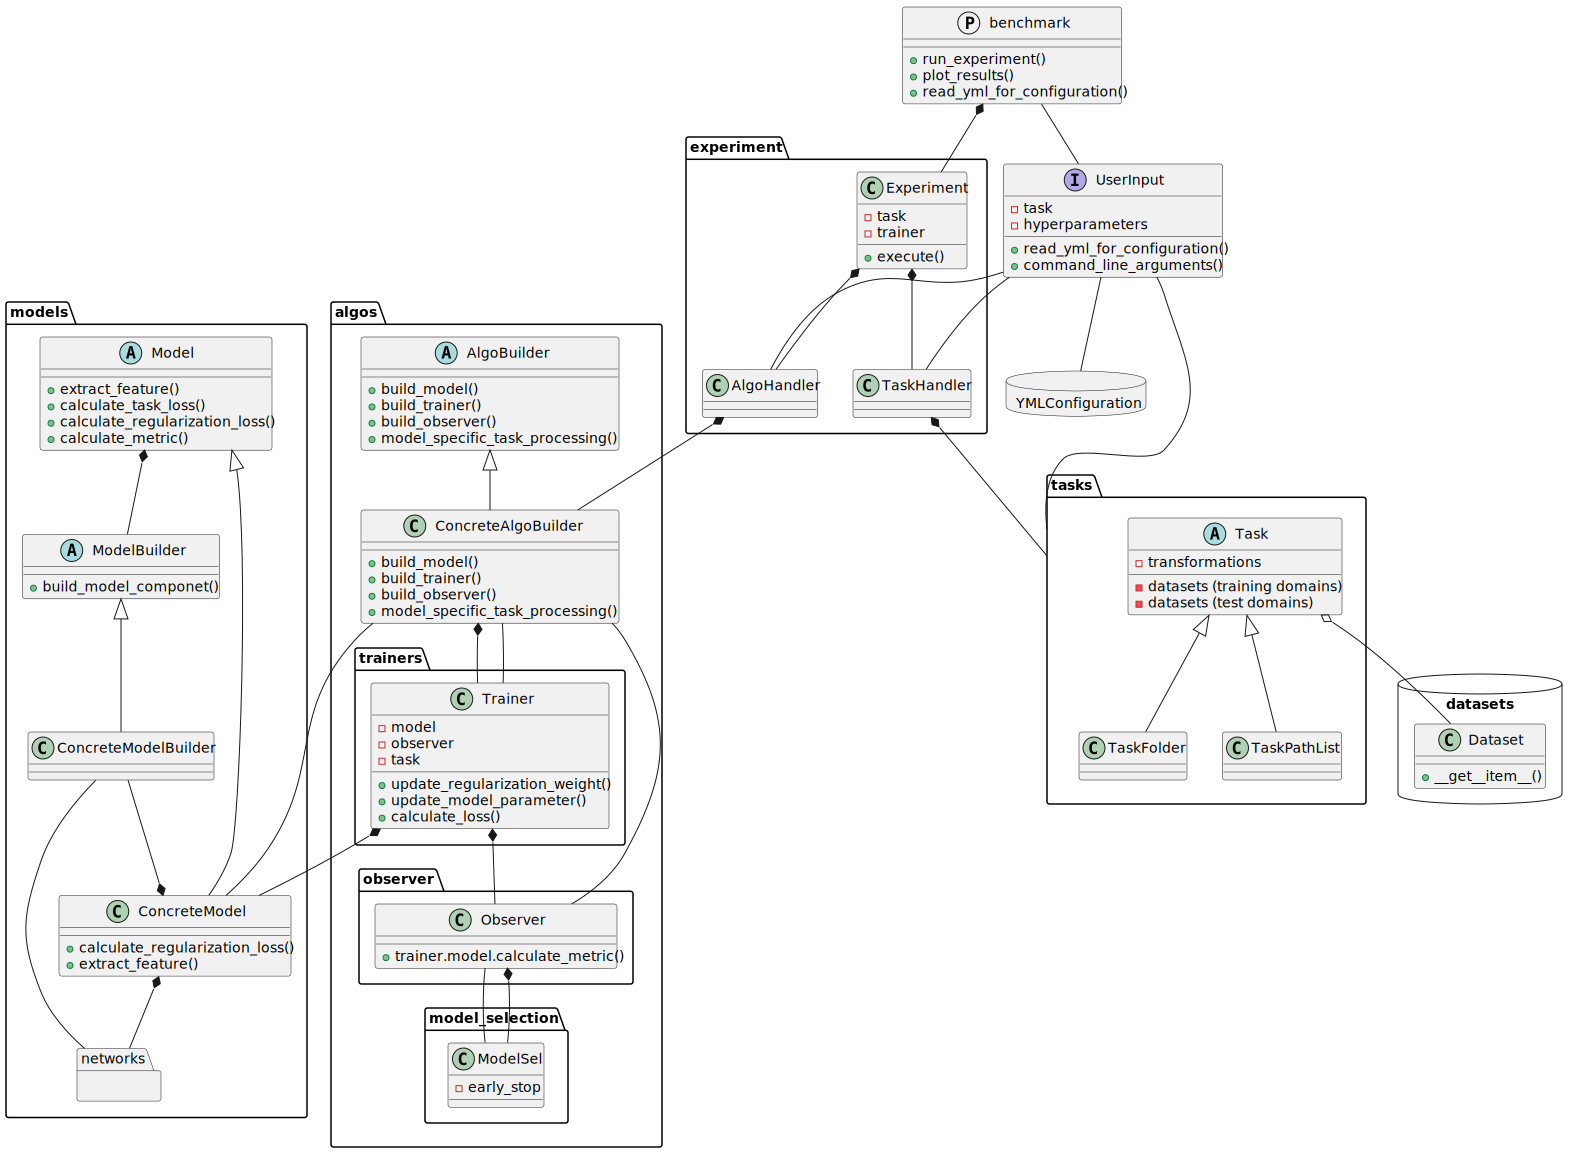
\includegraphics{../docs/libDG.svg}
\caption{DomainLab design architecture~\label{fig:cdiagram}}
\end{figure}

\hypertarget{availability}{%
\section{Availability}\label{availability}}

Domainlab is open source and freely available. It is published under the
MIT License. Users can download the source code at
\url{https://github.com/marrlab/DomainLab}. Extensive documentation can
be found here at \url{https://marrlab.github.io/DomainLab}. DomainLab
can be installed using the
\href{https://python-poetry.org/}{python-poetry} or
\href{https://pypi.org/project/pip/}{pip} utilities.

